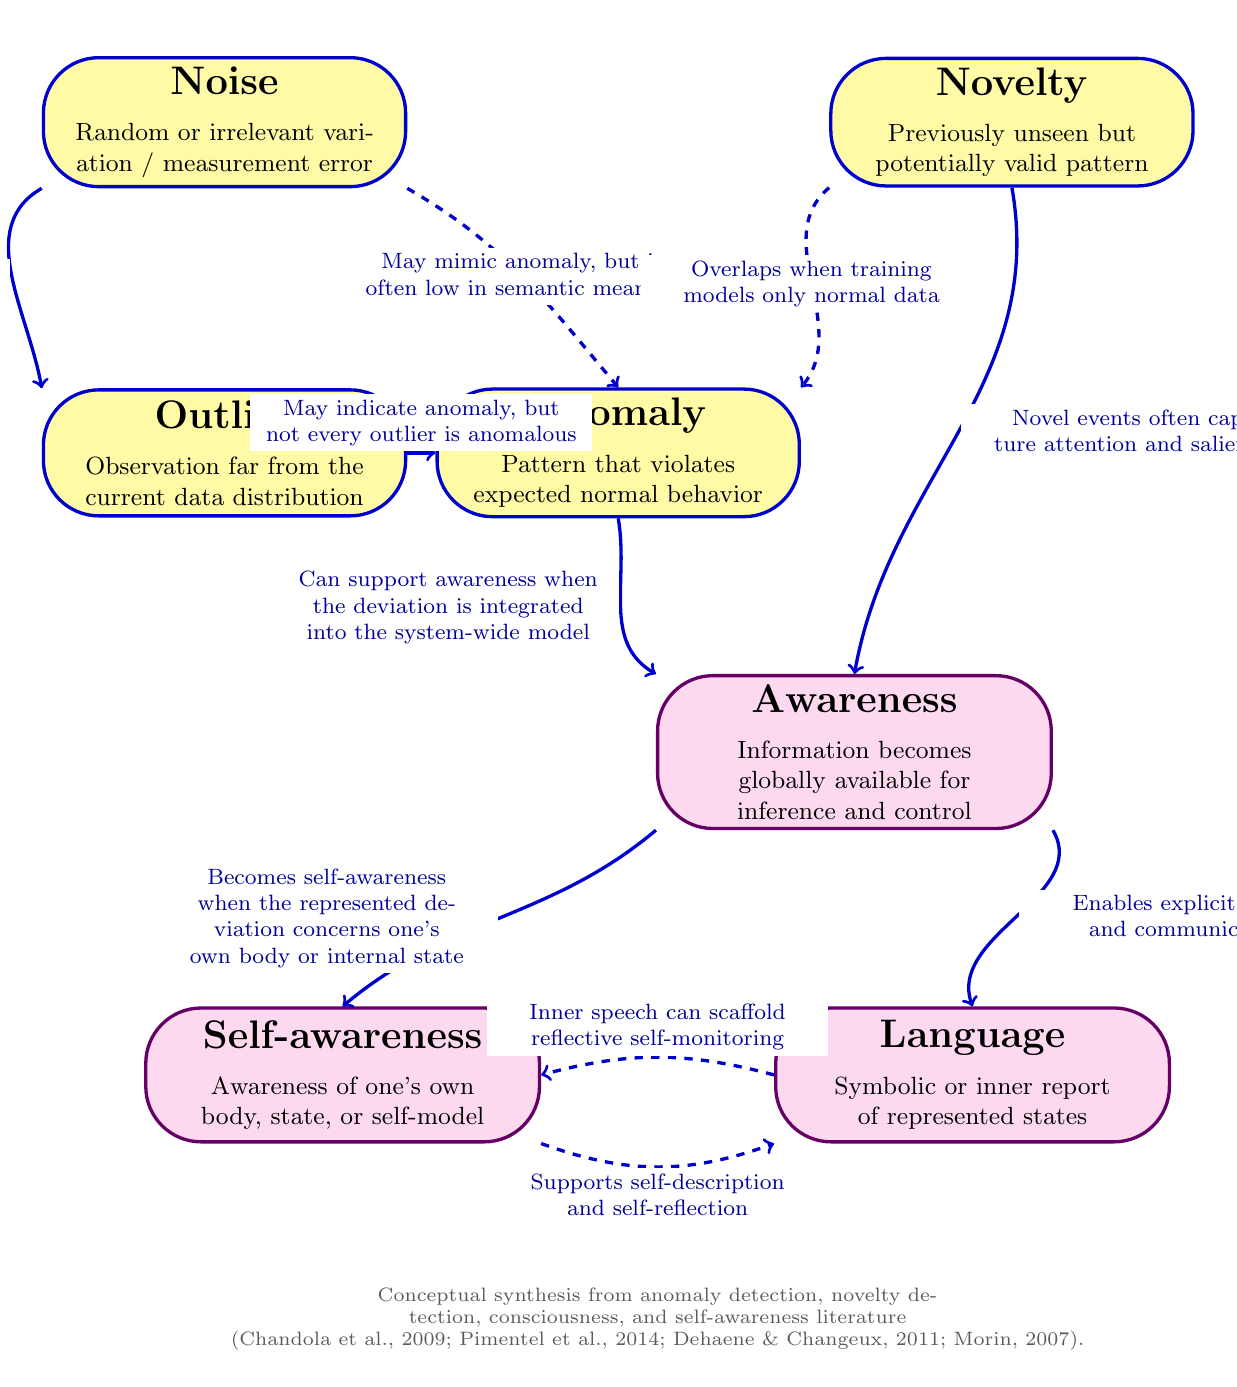
\begin{tikzpicture}[
    every node/.style={
        font=\small,
        align=center
    },
    statistical/.style={
        draw=blue!80!black,
        very thick,
        rounded corners=20pt,
        fill=yellow!35,
        minimum width=4.6cm,
        minimum height=1.6cm,
        text width=4.0cm
    },
    cognitive/.style={
        draw=violet!80!black,
        very thick,
        rounded corners=20pt,
        fill=magenta!15,
        minimum width=5.0cm,
        minimum height=1.7cm,
        text width=4.4cm
    },
    relation/.style={
        ->,
        very thick,
        blue!80!black
    },
    conditional/.style={
        ->,
        very thick,
        dashed,
        blue!80!black
    },
    relationlabel/.style={
        fill=white,
        inner sep=2pt,
        text=blue!60!black,
        font=\footnotesize,
        text width=4.2cm,
        align=center
    }
]

\useasboundingbox (-7.5,-15.7) rectangle (7.5,1.2);

\node[statistical] (noise) at (-5,0) {
    \textbf{\Large Noise}\\[2mm]
    Random or irrelevant variation / measurement error
};

\node[statistical] (novelty) at (5,0) {
    \textbf{\Large Novelty}\\[2mm]
    Previously unseen but potentially valid pattern
};

\node[statistical] (outlier) at (-5,-4.2) {
    \textbf{\Large Outlier}\\[2mm]
    Observation far from the current data distribution
};

\node[statistical] (anomaly) at (0,-4.2) {
    \textbf{\Large Anomaly}\\[2mm]
    Pattern that violates expected normal behavior
};

\node[cognitive] (awareness) at (3,-8) {
    \textbf{\Large Awareness}\\[2mm]
    Information becomes globally available for inference and control
};

\node[cognitive] (selfawareness) at (-3.5,-12.1) {
    \textbf{\Large Self-awareness}\\[2mm]
    Awareness of one's own body, state, or self-model
};

\node[cognitive] (language) at (4.5,-12.1) {
    \textbf{\Large Language}\\[2mm]
    Symbolic or inner report of represented states
};

\draw[relation]
    (noise.south west)
    to[out=210,in=100]
    node[relationlabel, left] {
        Can create spurious outliers
    }
    (outlier.north west);

\draw[conditional]
    (noise.south east)
    to[out=-30,in=130]
    node[relationlabel] {
        May mimic anomaly, but is often low in semantic meaning
    }
    (anomaly.north);

\draw[relation]
    (outlier.east)
    --
    node[relationlabel, above] {
        May indicate anomaly, but not every outlier is anomalous
    }
    (anomaly.west);

\draw[conditional]
    (novelty.south west)
    to[out=220,in=50]
    node[relationlabel] {
        Overlaps when training models only normal data
    }
    (anomaly.north east);

\draw[relation]
    (novelty.south)
    to[out=-80,in=80]
    node[relationlabel, right] {
        Novel events often capture attention and salience
    }
    (awareness.north);

\draw[relation]
    (anomaly.south)
    to[out=-80,in=150]
    node[relationlabel, left] {
        Can support awareness when the deviation is integrated into the
        system-wide model
    }
    (awareness.north west);

\draw[relation]
    (awareness.south west)
    to[out=220,in=40]
    node[relationlabel, left] {
        Becomes self-awareness when the represented deviation concerns
        one's own body or internal state
    }
    (selfawareness.north);

\draw[relation]
    (awareness.south east)
    to[out=-60,in=110]
    node[relationlabel, right] {
        Enables explicit report and communication
    }
    (language.north);

\draw[conditional]
    (language.west)
    to[out=165,in=15]
    node[relationlabel, above] {
        Inner speech can scaffold reflective self-monitoring
    }
    (selfawareness.east);

\draw[conditional]
    (selfawareness.south east)
    to[out=-20,in=200]
    node[relationlabel, below] {
        Supports self-description and self-reflection
    }
    (language.south west);

\node[
    font=\scriptsize,
    text width=13cm,
    align=center,
    text=black!65
] at (0.5,-15.2) {
    Conceptual synthesis from anomaly detection, novelty detection,
    consciousness, and self-awareness literature\\
    (Chandola et al., 2009; Pimentel et al., 2014;
    Dehaene \& Changeux, 2011; Morin, 2007).
};

\end{tikzpicture}